\documentclass{beamer}

\usepackage{textpos}
%\usepackage[spanish]{babel} % Manejo de idiomas
\usepackage[utf8]{inputenc} % Escritura en castellano con acent
%\usetheme{AnnArbor}
%\usetheme{Antibes}
%\usetheme{Bergen}
%\usetheme{Berkeley}
%\usetheme{Berlin}
%\usetheme{Boadilla}
%\usetheme{boxes}
%\usetheme{CambridgeUS}
%\usetheme{Copenhagen}
%\usetheme{Darmstadt}
%\usetheme{default}
%\usetheme{Frankfurt}
%\usetheme{Goettingen}
%\usetheme{Hannover}
%\usetheme{Ilmenau}
%\usetheme{JuanLesPins}
%\usetheme{Luebeck}
\usetheme{Madrid}
%\usetheme{Malmoe}
%\usetheme{Marburg}
%\usetheme{Montpellier}
%\usetheme{PaloAlto}
%\usetheme{Pittsburgh}
%\usetheme{Rochester}
%\usetheme{Singapore}
%\usetheme{Szeged}
%\usetheme{Warsaw}
\usecolortheme{beaver}
\usepackage{ragged2e}

\usepackage{listings}


\title[Data Science]{GraphQL, Apollo and Neo4j using React}

% A subtitle is optional and this may be deleted
%\subtitle{Los tres paradigmas de las ciencias de la computación \\(Amnon H. Eden, 2007 Springer Science+Bussines Media )}


%\author{MCC Miguel Ángel Uc Dzib}
\author[]{Jorge Rios\\Miguel Uc}


\institute[Ksquare Labs] % (optional, but mostly needed)
{		
	\date{\today}
	
	
	
	}

\titlegraphic{
	
	
\includegraphics[width=2cm]{img/ksquare.png}
%	\hspace*{3.75cm}~%
	%\includegraphics[width=3cm]{img/fmatLogo.png}
}


\AtBeginSection[]
{
	\frame<handout:0>
	{
		\frametitle{}
		\tableofcontents[currentsection,hideallsubsections]
	}
}




\begin{document}

\begin{frame}
 \titlepage
\end{frame}

\begin{frame}{Contents}
	\tableofcontents
	% You might wish to add the option [pausesections]
\end{frame}
\addtobeamertemplate{frametitle}{}{\begin{textblock*}{100mm}(.9\textwidth,-0.9cm)
\includegraphics[width=0.15\linewidth]{img/ksquare.png}\end{textblock*}}


\section{Schemma postgresql}
\begin{frame}{Schemma postgresql}{ }
We will be using the NorthWind dataset, a commonly-used SQL dataset. Although the NorthWind dataset is often used to demonstrate SQL and relational databases, it is graphy enough to be interesting for us. 

\end{frame}


\begin{frame}{Schemma postgresql}{ }
\begin{itemize}
	\item The following is an entity-relationship diagram of the Northwind dataset:
\end{itemize}	
\begin{center}
	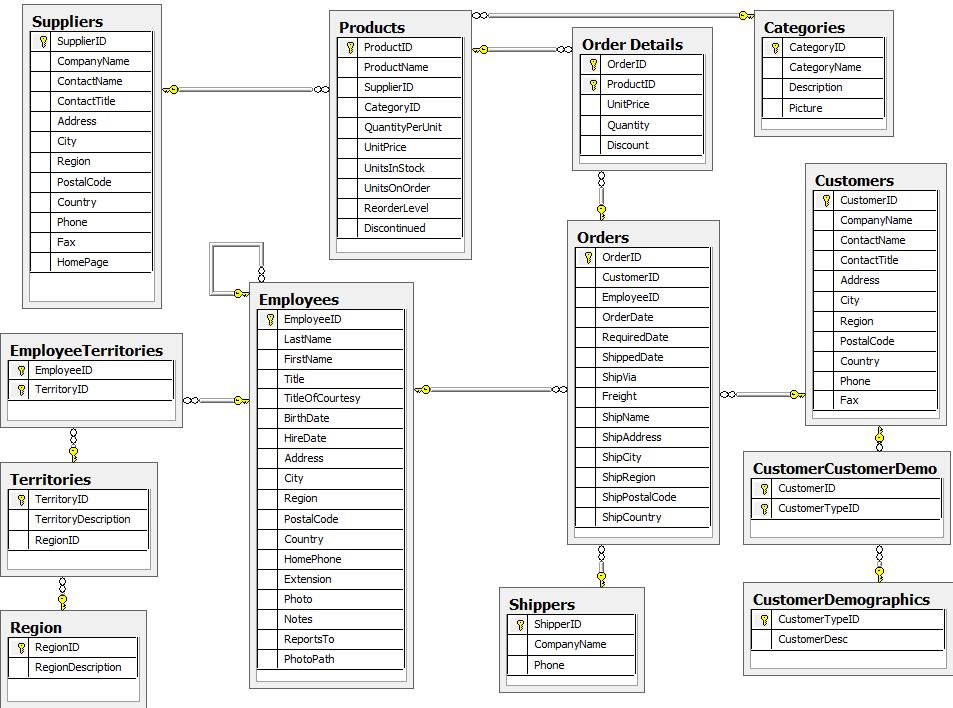
\includegraphics[width=0.7\linewidth]{img/Northwind_diagram.jpg}
\end{center}
\end{frame}

\begin{frame}{Schemma postgresql}{ }	
\begin{center}
	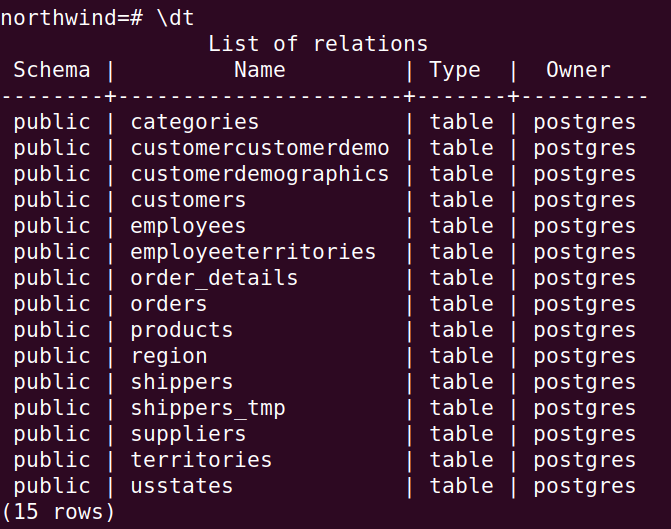
\includegraphics[width=0.7\linewidth]{img/postgresql.png}
\end{center}
\end{frame}


\section{Schema Neo4j}

\begin{frame}{Schema Neo4j}{ }
	When deriving a graph model from a relational model, we should keep the following guidelines in mind:
\begin{itemize}	

		\item A row is a node
		\item A table name is a label name
\end{itemize}

\end{frame}

\begin{frame}{Schema Neo4j}{ }
	The following graph model represent the Northwind dataset:	
\begin{center}
	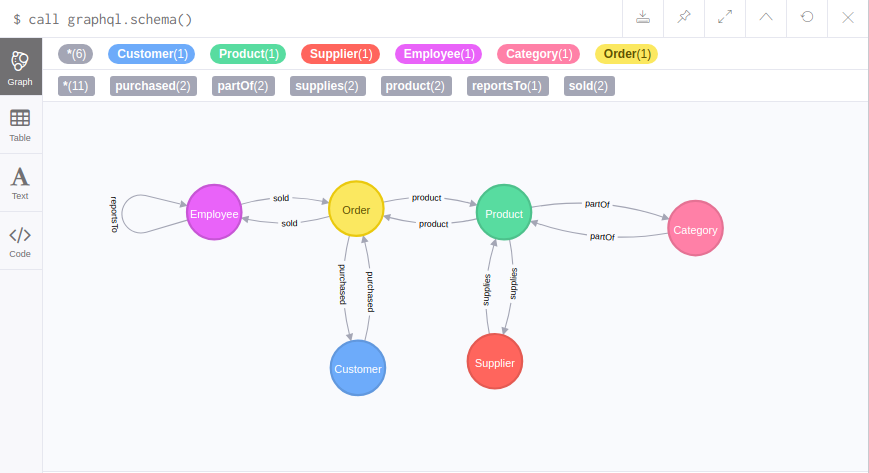
\includegraphics[width=1.0\linewidth]{img/graph.png}
\end{center}
\end{frame}

\section{Apollo}
\begin{frame}{Apollo}{ }
\begin{itemize}
	\item Apollo is a family of technologies you can incrementally add to your stack: Apollo Client to connect data to your UI, Apollo Engine for infrastructure and tooling, and Apollo Server to translate your REST API and backends into a GraphQL schema.
\end{itemize}

\begin{center}
	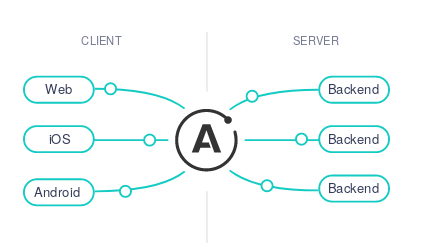
\includegraphics[width=0.7\linewidth]{img/apollo.png}
\end{center}
\end{frame}

\section{GraphQL}

\begin{frame}{GraphQL}{ }
	\begin{itemize}
		\item GraphQL is a query language for your API, and a server-side runtime for executing queries by using a type system you define for your data.
		\item  For example, a GraphQL service that tells us who the logged in user is (me) as well as that user's name might look something like this:
	\end{itemize}

\begin{center}
	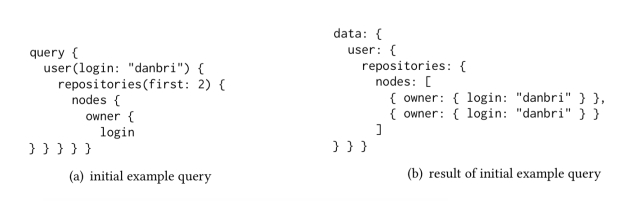
\includegraphics[width=0.7\linewidth]{img/query.jpeg}
\end{center}
\end{frame}





\section{Aplication}

\begin{frame}{Aplication}{ }
\begin{itemize}
	\item This project is a starter for building a GraphKsquare (GraphQL, React, Apollo, Neo4j Database) application. There are two components to the starter, the UI application (a React app) and the API app (GraphQL server).
\end{itemize}
\end{frame}

\begin{frame}{Aplication}{ }
\begin{itemize}
	\item This project is a starter for building a GraphKsquare (GraphQL, React, Apollo, Neo4j Database) application. There are two components to the starter, the UI application (a React app) and the API app (GraphQL server).
\end{itemize}
\end{frame}

\begin{frame}{Aplication}{ }

\begin{center}
	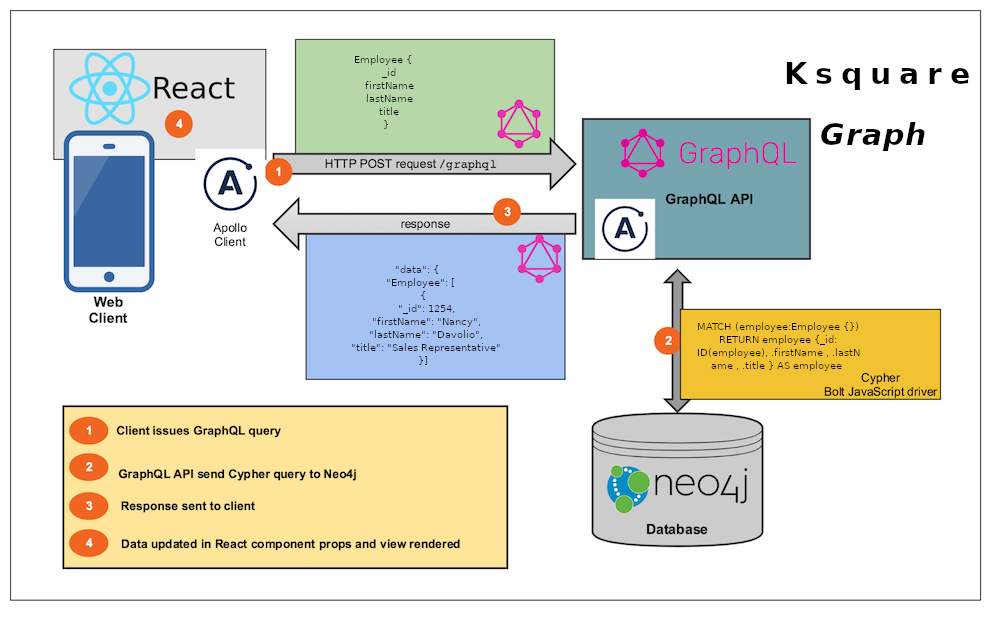
\includegraphics[width=0.7\linewidth]{img/neoapographqla.png}
\end{center}
\end{frame}


\begin{frame}{API input}{ }

\begin{center}
	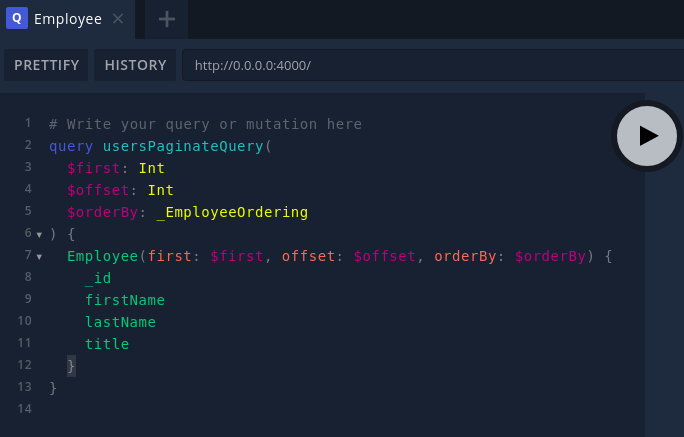
\includegraphics[width=0.7\linewidth]{img/graphqlinput.png}
\end{center}
\end{frame}

\begin{frame}{API output}{ }

\begin{center}
	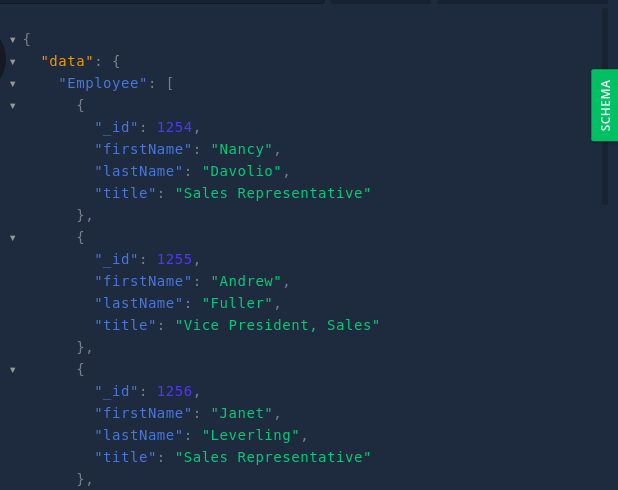
\includegraphics[width=0.7\linewidth]{img/graphqloutput.png}
\end{center}
\end{frame}

\begin{frame}{UI application}{ }

\begin{center}
	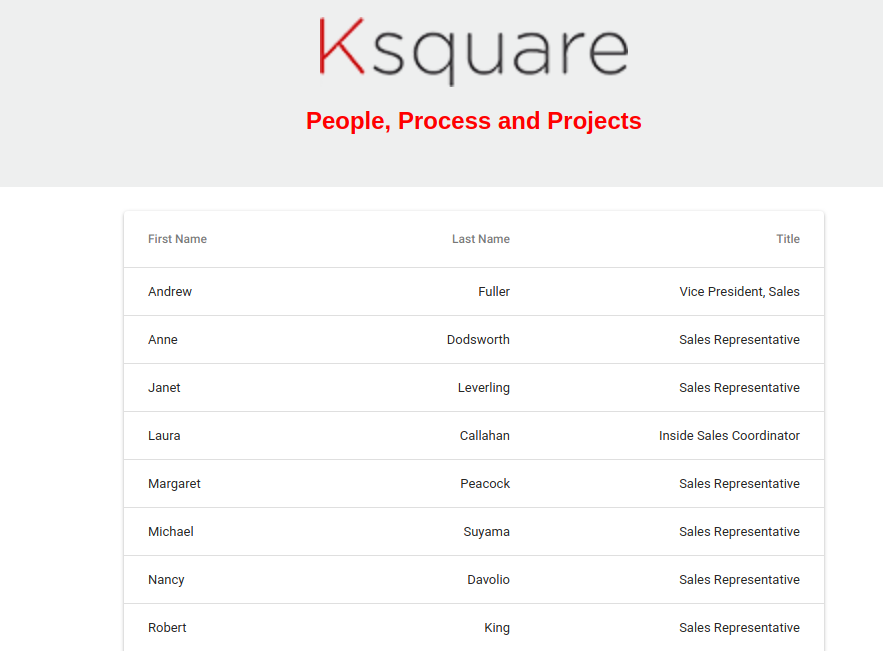
\includegraphics[width=0.7\linewidth]{img/reactoutput.png}
\end{center}
\end{frame}


\begin{frame}{About Security}{ }

\begin{itemize}
\item Denial of Service Attack.
		\begin{enumerate}
		\item Whitelist of queries using Apollo's persistgraphql
		\item Depth limiting using  graphql-depth-limit
		\item Amount limiting (99999) with custom scalar created with graphql-input-number
		\item Query Cost Analysis with graphql-cost-analysis (Mutations are hard to estimate)
		\end{enumerate}
		 
		 
\end{itemize}
\end{frame}

\begin{frame}{About Security 2}
An example of security scheme is the one used by GitHub:
\begin{itemize}
\item Token based authentication (or bearer authentication). It can be applied to operation level. It can use JWT format.
\item Clients must supply a first or last argument on any connection.
\item Values of first and last must be within 1-100.
\item Individual calls cannot request more than 500,000 total nodes.
\item Rate limit is 5,000 points per hour. A formula is applied to each query on parent and children arguments.


\end{itemize} 
\end{frame}

\section{Referencias}
\begin{frame}{Referencias}
  \begin{thebibliography}{10} 	
  	\beamertemplatearticlebibitems
  	
  	\bibitem{wombat2016}
  	   \url{https://graphql.org/learn/}		
  	\bibitem{wombat2017}
  	\url{https://www.apollographql.com/}
  	\bibitem{wikibook} 
  	\url{https://neo4j.com/blog/}
  	\bibitem{grandstack}
  	\url{https://grandstack.io/}
  	\bibitem{github}
  	\url{https://developer.github.com}
  \end{thebibliography}
\end{frame}

\end{document}